% Authored By Shashank Shantharam Nayak

% Define commands for each person
\newcommand{\pOne}{EDGAR ALLAN POE (1BMXXYYZZZZ)}
\newcommand{\pTwo}{SHERLOCK HOLMES (1BMXXYYZZZZ)}
\newcommand{\pThree}{ALEXANDER GRAHAM BELL (1BMXXYYZZZZ)}
\newcommand{\pFour}{HERCULE POIROT (1BMXXYYZZZZ)}
\newcommand{\semester}{3rd}

\newcommand{\projName}{SKILL-IT}
\newcommand{\subject}{Full Stack Web Development}
\newcommand{\subjectCode}{23CS3AEFWD}
\newcommand{\academicSemester}{Even}
\newcommand{\academicYear}{2024 - 2025}

\newcommand{\guide}{GUIDE NAME}
\newcommand{\guideDesg}{Designation}
\newcommand{\HOD}{Dr. Kavitha Sooda}
\newcommand{\principal}{Dr. Bheemsha Arya}

\PassOptionsToPackage{unicode}{hyperref}
\PassOptionsToPackage{hyphens}{url}
\PassOptionsToPackage{dvipsnames,svgnames,x11names}{xcolor}
\documentclass[
  12pt,
  a4paper,
  ]{report}
\usepackage{xcolor}
\usepackage[left=1in,right=1in,top=1in,bottom=1in]{geometry}
\usepackage{amsmath,amssymb}
\setcounter{secnumdepth}{3}
\usepackage{iftex}
\usepackage{graphicx}
\usepackage{tabulary}
\usepackage{lipsum}
\usepackage{tikz}
\hyphenpenalty=10000
\sloppy
\ifPDFTeX
  \usepackage[T1]{fontenc}
  \usepackage[utf8]{inputenc}
  \usepackage{textcomp} % provide euro and other symbols
\else % if luatex or xetex
  \usepackage{unicode-math} % this also loads fontspec
  \defaultfontfeatures{Scale=MatchLowercase}
  \defaultfontfeatures[\rmfamily]{Ligatures=TeX,Scale=1}
\fi
\usepackage{lmodern}
\usepackage[backend=biber, style=alphabetic]{biblatex}
\addbibresource{references.bib}
\IfFileExists{microtype.sty}{% use microtype if available
  \usepackage[]{microtype}
  \UseMicrotypeSet[protrusion]{basicmath} % disable protrusion for tt fonts
}{}
\usepackage{setspace}
\makeatletter
\@ifundefined{KOMAClassName}{% if non-KOMA class
  \IfFileExists{parskip.sty}{%
    \usepackage{parskip}
  }{% else
    \setlength{\parindent}{0pt}
    \setlength{\parskip}{6pt plus 2pt minus 1pt}}
}{% if KOMA class
  \KOMAoptions{parskip=half}}
\makeatother
\usepackage{longtable,booktabs,array}
\usepackage{calc} % for calculating minipage widths
% Correct order of tables after \paragraph or \subparagraph
\usepackage{etoolbox}
\makeatletter
\patchcmd\longtable{\par}{\if@noskipsec\mbox{}\fi\par}{}{}
\makeatother
% Allow footnotes in longtable head/foot
\IfFileExists{footnotehyper.sty}{\usepackage{footnotehyper}}{\usepackage{footnote}}
\makesavenoteenv{longtable}
\setlength{\emergencystretch}{3em} % prevent overfull lines
\providecommand{\tightlist}{%
  \setlength{\itemsep}{0pt}\setlength{\parskip}{0pt}}
\makeatletter
\@ifpackageloaded{subfig}{}{\usepackage{subfig}}
\@ifpackageloaded{caption}{}{\usepackage{caption}}
\captionsetup[subfloat]{margin=0.5em}
\AtBeginDocument{%
\renewcommand*\figurename{Figure}
\renewcommand*\tablename{Table}
}
\AtBeginDocument{%
\renewcommand*\listfigurename{List of Figures}
\renewcommand*\listtablename{List of Tables}
}
\newcounter{pandoccrossref@subfigures@footnote@counter}
\newenvironment{pandoccrossrefsubfigures}{%
\setcounter{pandoccrossref@subfigures@footnote@counter}{0}
\begin{figure}\centering%
\gdef\global@pandoccrossref@subfigures@footnotes{}%
\DeclareRobustCommand{\footnote}[1]{\footnotemark%
\stepcounter{pandoccrossref@subfigures@footnote@counter}%
\ifx\global@pandoccrossref@subfigures@footnotes\empty%
\gdef\global@pandoccrossref@subfigures@footnotes{{##1}}%
\else%
\g@addto@macro\global@pandoccrossref@subfigures@footnotes{, {##1}}%
\fi}}%
{\end{figure}%
\addtocounter{footnote}{-\value{pandoccrossref@subfigures@footnote@counter}}
\@for\f:=\global@pandoccrossref@subfigures@footnotes\do{\stepcounter{footnote}\footnotetext{\f}}%
\gdef\global@pandoccrossref@subfigures@footnotes{}}
\@ifpackageloaded{float}{}{\usepackage{float}}
\floatstyle{ruled}
\@ifundefined{c@chapter}{\newfloat{codelisting}{h}{lop}}{\newfloat{codelisting}{h}{lop}[chapter]}
\floatname{codelisting}{Listing}
\newcommand*\listoflistings{\listof{codelisting}{List of Listings}}
\makeatother
\usepackage{bookmark}
\IfFileExists{xurl.sty}{\usepackage{xurl}}{} % add URL line breaks if available
\urlstyle{same}
\hypersetup{
  pdfkeywords={Keyword1, Keyword2, Keyword3},
  colorlinks=true,
  linkcolor={Maroon},
  filecolor={Maroon},
  citecolor={Blue},
  urlcolor={Blue},
  pdfcreator={LaTeX via pandoc}}

\begin{document}

\pagenumbering{roman}

% Title Page
\begin{titlepage}
    \centering
    
    % Place for VTU Logo
    \textbf{
    {\large VISVESVARAYA TECHNOLOGICAL}\\[0.5em]
    {\large UNIVERSITY}}\\[0.5em]
    {\large “Jnana Sangama”, Belgaum -590014, Karnataka} \\
    
    \vspace*{0.5cm}
    
\includegraphics[width=0.15\textwidth]{vtu.png} \\

    \vspace{0.5cm}
    
    {\large \textbf{FULL STACK WEB DEVELOPMENT}}\\[0.5em]
    {\large \textbf{PROJECT REPORT}} \\
    \vspace{0.25cm}
    {\large On} \\
    \vspace{0.5cm}
    {\Large \textbf{“SKILL – IT”}} \\
    
    \vspace{0.5cm}
    
    {\large Submitted by} \\
    \vspace{0.5cm}
    \textbf{
    {\large SHERLOCK HOLMES (1BMXXYYZZZZ)} \\
    {\large ALEXANDER GRAHAM BELL (1BMXXYYZZZZ)} \\
    {\large HERCULE POIROT (1BMXXYYZZZZ)} \\
    {\large EDGAR ALLAN POE (1BMXXYYZZZZ)} \\
    }
    \vspace{0.75cm}
    
    {\large Under the Guidance of} \\
    \textbf{
    {\large YOUR GUIDE}\\
    {\large Designation} \\
    }
    \vspace{0.5cm}
    
    {\large in partial fulfillment for the award of the degree of} \\
    \vspace{0.5cm}
    {\large \textbf{BACHELOR OF ENGINEERING}} \\
    \vspace{0.125cm}
    {\large in} \\
    \vspace{0.25cm}
    {\large \textbf{COMPUTER SCIENCE AND ENGINEERING}} \\
    
    \vspace{1cm}
    
    
\includegraphics[width=0.15\textwidth]{bmsce.png} \\
    \vspace{0.5cm}
    {\large \textbf{B.M.S. COLLEGE OF ENGINEERING}} \\[0.5em]
    {\large (Autonomous Institution under VTU)} \\[0.5em]
    { BENGALURU-560019} \\[0.5em]
    { 2024-2025} \\
    
    % Place for BMSCE Logo

\end{titlepage}

\clearpage


    \begin{center}
    
    {\large \textbf{B. M. S. College of Engineering,}}\\[0.25em]
    {\large \textbf{Bull Temple Road, Bengaluru 560019}}\\[0.25em]
    
    (Affiliated To Visvesvaraya Technological University, Belgaum)\\[0.25em]
    \textbf{Department of Computer Science and Engineering}
        

    \vspace{0.75cm}
    
\includegraphics[width=0.15\textwidth]{bmsce.png}\\
    \vspace{0.75cm}
    \textbf{\Large \underline{CERTIFICATE}}\\
    \vspace{0.5cm}
    \end{center}

    \begin{spacing}{1.25}
    \noindent
    {\large This is to certify that the project work entitled 
    \textbf{“SKILL-IT”},
    carried out by \textbf{SHERLOCK HOLMES (1BMXXYYZZZZ), ALEXANDER GRAHAM BELL (1BM23CS313), HERCULE POIROT (1BM23CS340), EDGAR ALLAN POE (1BM23CS348)}, bonafide students of \textbf{B. M. S. College of Engineering}, is in partial fulfillment for the award of Bachelor of Engineering in Computer Science and Engineering of Visvesvaraya Technological University, Belgaum during the year 2024 and satisfies the academic requirements of the course Full Stack Web Development (23CS3AEFWD) prescribed for the said degree.
    
    \vspace{2cm}

    \setlength\tabcolsep{0pt}
    \noindent
    \begin{tabular*}{\linewidth}{@{\extracolsep{\fill}} lr }
    \textbf{YOUR GUIDE} & \textbf{Name of HOD} \\
    Designation   & Professor and Head \\
    B. M. S. College of Engineering   & Department of CSE \\
    Bengaluru & B. M. S. College of Engineering \\
    & Bengaluru \\
    \end{tabular*}
    
    \vspace{2cm}  % Add vertical space between the tables
    
    \noindent
    \setlength\tabcolsep{0pt}
    \noindent
    \begin{tabular*}{\linewidth}{@{\extracolsep{\fill}} lr }
    Name of the Examiner & Signature with Date\\
    \end{tabular*}
    
    }
    \end{spacing}

\clearpage

    \begin{center}
    
    {\large \textbf{B. M. S. College of Engineering,}}\\[0.25em]
    {\large \textbf{Department of Computer Science and Engineering}}

    \vspace{0.75cm}
    
\includegraphics[width=0.15\textwidth]{bmsce.png}\\
    \vspace{0.75cm}
    
    \textbf{\Large \underline{Declaration}}\\
    \vspace{0.5cm}
    \end{center}

    \begin{spacing}{1.25}
        
        \noindent
        \large We, \textbf{SHERLOCK HOLMES (1BMXXYYZZZZ), ALEXANDER GRAHAM BELL (1BM23CS313), HERCULE POIROT (1BM23CS340), EDGAR ALLAN POE (1BM23CS348)}, students of \textbf{3rd Semester, B.E, Department of Computer Science and Engineering, BMS College of Engineering, Bengaluru}, hereby declare that this Full Stack Web Development project entitled \textbf{"Skill-It"} has been carried out by us under the guidance of \textbf{YOUR GUIDE}, Designation, Department of CSE, B.M.S College of Engineering, Bangalore, during the academic semester \textbf{Sept 2024 - Jan 2025}.

        \noindent
        \Large We also declare that, to the best of our knowledge and belief, the development reported here is not a part of any other report by any other students.
        
        \vspace{1cm}
        \setlength\tabcolsep{0pt}
        \noindent
        \begingroup
        \fontsize{14pt}{12pt}
        \begin{tabulary}{0.95\linewidth}{LR}
            & Signatures \\
            \textbf{SHERLOCK HOLMES (1BMXXYYZZZZ)} & \\
            \textbf{ALEXANDER GRAHAM BELL (1BMXXYYZZZZ)} & \\
            \textbf{HERCULE POIROT (1BMXXYYZZZZ)} & \\
            \textbf{EDGAR ALLAN POE (1BMXXYYZZZZ)} & \\
        \end{tabulary}
        \endgroup
    \end{spacing}
\clearpage
    \begin{center}
    \Large \textbf{ABSTRACT}
    \end{center}
    \begin{spacing}{2.0}
        \lipsum[0-5]
    \end{spacing}


\renewcommand*\contentsname{Table of Contents}
{
\hypersetup{linkcolor=blue}
\setcounter{tocdepth}{2}
\tableofcontents
}
\listoffigures
\listoftables
\setstretch{1.5}
\clearpage
\pagenumbering{arabic}
\chapter{Introduction to Quantum Computing}\label{chap1}

Quantum computing is an advanced area of computation that relies on the
principles of quantum mechanics to process information in fundamentally
different ways than classical computers. Traditional computers represent
data as binary digits (bits), which can exist in one of two states: 0 or
1. Quantum computers, on the other hand, use quantum bits (qubits),
which can exist in multiple states simultaneously due to the phenomena
of superposition and entanglement.

This ability allows quantum computers to solve specific types of
problems much faster than classical computers. Problems involving large
datasets, complex simulations (such as molecular chemistry),
optimization, and machine learning could see major improvements in speed
and accuracy with the use of quantum algorithms.

As Peter Shor said:

\begin{quote}
In the near future, quantum computers may be able to break widely used
encryption systems, but they will also create new, far stronger
encryption methods.
\end{quote}

\section{The Foundation of Quantum Computing}\label{foundation}

As referenced in \href{chap1}{Introduction} above, Quantum computing is
based on the fundamental principles of quantum mechanics, the branch of
physics that describes the behavior of particles at the subatomic level.
Three key concepts from quantum mechanics form the foundation of quantum
computing:

\begin{enumerate}
\def\labelenumi{\arabic{enumi}.}
\item
  Superposition: A quantum system can exist in a linear combination (or
  superposition) of multiple states at once. For instance, whereas a
  classical bit can only be in the state 0 or 1, a qubit can be in a
  state that is a combination of both 0 and 1. This enables quantum
  computers to process a vast amount of information in parallel.
\item
  Entanglement: When two qubits are entangled, their states become
  interconnected, meaning that changing one qubit will instantly affect
  the other, regardless of the distance between them. This phenomenon
  can be used to create highly parallelized computational processes,
  accelerating problem-solving in quantum algorithms.
\item
  Quantum Interference: Quantum algorithms make use of interference to
  amplify the probability of correct answers and cancel out wrong ones.
  By manipulating the phase of the quantum state, quantum computers
  enhance the likelihood of achieving the correct solution while
  eliminating errors. Some random Code
  \texttt{python\ \ \ \ \ \ \ \ \ s\ =\ "HI"\ \ \ \ \ \ \ \ \ if\ s\ ==\ "HI":\ \ \ \ \ \ \ \ \ \ \ \ \ print(s)}
\end{enumerate}

\begin{description}
\item[Qubit:]
A qubit (short for quantum bit) is the basic unit of information in
quantum computing. Unlike a classical bit, which can only represent one
of two possible states, 0 or 1, a qubit can represent both 0 and 1
simultaneously due to a property called superposition.
\end{description}

Pandoc supports task lists, using the syntax of GitHub-Flavored
Markdown.

\begin{itemize}
\tightlist
\item[$\square$]
  an unchecked task list item
\item[$\boxtimes$]
  checked item
\end{itemize}

\begin{center}\rule{0.5\linewidth}{0.5pt}\end{center}

\chapter{Mathematical Foundation to Quantum Computing}\label{chap1}

\lipsum[0-5]

\chapter{The Architecture of Quantum
Computing}\label{the-architecture-of-quantum-computing}

\begin{center}
\begin{tikzpicture}[shorten >=1pt, node distance=2cm, auto]
    \node (A) {A};
    \node (B) [right of=A] {B};
    \node (C) [right of=B] {C};
    \node (D) [below of=A] {D};

    \path[->] 
        (A) edge (B)
        (B) edge (C)
        (C) edge (B)
        (A) edge (D);
\end{tikzpicture}
\label{GraphRef}
\end{center}

\begin{longtable}[]{@{}llll@{}}
\caption{Caption \{\#tbl:tabRef\}}\tabularnewline
\toprule\noalign{}
ID & Name & Age & Country \\
\midrule\noalign{}
\endfirsthead
\toprule\noalign{}
ID & Name & Age & Country \\
\midrule\noalign{}
\endhead
\bottomrule\noalign{}
\endlastfoot
1 & Alice & 24 & USA \\
2 & Bob & 30 & Canada \\
3 & Charlie & 22 & UK \\
4 & David & 28 & Australia \\
5 & Emma & 35 & Germany \\
6 & Frank & 27 & France \\
\end{longtable}

\[ x^2 + y^2 = c^2 \]

Above equation given by \autocite{Einstein1905}.

This is a citation to the work of Smith et al. \autocite{smith2021}.

\begin{figure}
\centering
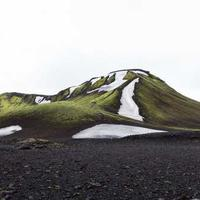
\includegraphics{./resources/img.jpg}
\caption{My Image}\label{fig:imgRef}
\end{figure}
\printbibliography
\end{document}
